\documentclass[a4paper,11pt]{article}
\usepackage[utf8]{inputenc}
\usepackage{lmodern}
\usepackage[T1]{fontenc}
\usepackage[pdftex]{hyperref}
\usepackage{eurosym}
\usepackage{scrextend}
\usepackage{graphicx}
\usepackage{hyphenat}

\begin{document}

\begin{titlepage}
\title{\huge \textbf{Local Area Network Distributed Backup Service\\[1cm] \Large Enhancements specification\\[1cm] 
\includegraphics{logo.png}\\[1cm] \large Distributed Systems\\[0.25cm] \small $3^{rd}$ year\\[0.05cm]Master in Informatics and Computing Engineering\\[1.7cm]}\normalsize Class 4 - Group 7}

\author{José Peixoto\\Pedro Moura\\Paulo Costa\\Marina Camilo \and 200603103\\201306843\\201206045\\201307722 \and ei12134@fe.up.pt \\ up201306843@fe.up.pt\\ei12086@fe.up.pt\\up201307722@fe.up.pt\\[0.5cm]}
\maketitle
\thispagestyle{empty} % titlepage must not be numbered
\end{titlepage}

\newpage
\tableofcontents
\newpage

\section{Sub-protocols enhancements}

In order to simplify the development of the new security and scalability features, a code restructuring was made to make use of the sub-protocols enhancements described below as the default system for the peer communication. In short, retro-compatibility is now broken.

\subsection{Backup sub-protocol enhancement}
The default backup sub-protocol relies on sending a \texttt{PUTCHUNK} message to the \texttt{MDB} multicast data backup channel and replying with a \texttt{STORED} message for each chunk backed up without checking if any other peer had already stored it, resulting in excessive replication.

In order not to rapidly deplete the backup space available in all peers, the backup enhancement sub-protocol waits between 0 to 400 milliseconds allowing for the arrival of other peers \texttt{STORED} messages regarding that same chunk and compares the current and desired replication degrees to decide if it also needs to store it.

\subsubsection*{Peer-initiator}
\begin{verbatim}
while counter < 5
    send PUTCHUNK
    if received STORED count >= replicationDegree
        return
\end{verbatim}

\subsubsection*{Peer}
\begin{verbatim}
if received PUTCHUNK
    random delay 0-400 ms
    if currentReplicationDegree < desiredReplicationDegree
        store chunk
\end{verbatim}

This solution ensures a reduced over-replication of the chunks while still allowing for restoration.

\subsection{Restore sub-protocol enhancement}
The default restore sub-protocol relies on sending a \texttt{GETCHUNK} to the \texttt{MC} multicast control channel and waiting for a few milliseconds for new incoming messages containing the desired \texttt{CHUNK} to restore. According to the specification, ``each peer shall wait for a random time uniformly distributed between 0 and 400 ms, before sending the \texttt{CHUNK} message'', preventing overloading the \texttt{MDR} multicast data recovery channel.

In the enhanced version of this sub-protocol, the peer-initiator opens a server socket and binds it to a random \texttt{TCP} port and sends a \texttt{GETCHUNK} request with that port in the header to the multicast control channel. If the remote peer has the chunk, an attempt to establish a direct one-to-one reliable \texttt{TCP} connection is made, replacing the need for the \texttt{MDR} multicast data recovery channel for the \texttt{CHUNK} packet transit. Communicating in this manner also prevents other uninterested peers from receiving irrelevant \texttt{CHUNK} messages.

\subsubsection*{Peer-initiator}
\begin{verbatim} 
create socketChannel server
send GETCHUNK request to the MDC
if received the CHUNK
    store the CHUNK data
\end{verbatim}

\subsubsection*{Peer}
\begin{verbatim} 
if received GETCHUNK
    CHUNK = retrieveLocalChunk(fileID, chunkNo);
    if socketChannel connection is established
        send CHUNK
\end{verbatim}

\subsection{Delete sub-protocol enhancement}
In the default delete sub-protocol, a peer that received a \texttt{DELETE} request message shall remove from its backing store all the chunks belonging to the specified file.

The enhanced version adds a new confirmation message that is sent from the peers that successfully deleted their copies of the chunks: the \texttt{DELETEACK}.\\[0.1cm]

\texttt{DELETEACK <Version> <SenderId> <FileId> <CRLF><CRLF>}\\[0.1cm]

It uses the same format as the predefined delete message and allows the peer-initiator to count and compare the received confirmations of the \texttt{DELETE} request and expected file replication degree.

\subsubsection*{Peer-initiator}
\begin{verbatim} 
create thread
replicationDegree = chunkReplicationDegree
waitingTime = 15 seconds
while waitingTime < 16 minutes && replicationDegree > 0
    send DELETE
    replicationDegree -= DELETEACKS
    waitingTime *= 2
\end{verbatim}

\subsubsection*{Peer}
\begin{verbatim} 
if received DELETE
    delete chunks
    send DELETEACK
\end{verbatim}

\subsection{Reclaim sub-protocol enhancement}
The default reclaim sub-protocol attempts to delete some local chunks in order to free the requested disk space and communicates through the multicast control channel that it has removed the selected chunks, sending the \texttt{REMOVED} message. The other network peers, upon receiving the \texttt{REMOVED} message for a given chunk, compare the new replication degree of the chunk to its desired degree and in case the former is lower, the backup sub-protocol for that chunk might be initiated.

When the backup sub-protocol fails before its completion (both when a chunk is being backed up for the first time and when a copy of the chunk is deleted), the replication degree of the file might be lower than expected, effectively lowering its replication degree for some chunks. In the developed enhanced version, when a peer receives a \texttt{PUTCHUNK} request through the multicast data backup channel containing a chunk it has already backed up, a waiting period for the maximum backup sub-protocol time is made, followed by the re-initialization of the backup sub-protocol, this time by another peer, if the desired replication degree wasn't reached.

\subsection*{Peer}
\begin{verbatim} 
if received PUTCHUNK(c) && hasChunk(c)
    wait BACKUP_MAX_CONFIRMATION_WAIT;
    clearInbox();
    wait MAX_DELAY_MILLISECONDS;
if no PUTCHUNK(c) was received &&
        currentReplicationDegree < expectedReplicationDegree
    start backup(c)
\end{verbatim}

\section{Security}
Contrary to what was lectured, the security layer was in fact added as an after-thought. The developed security features described below attempt to provide integrity, authenticity and confidentiality when transmitting the chunks through the network.

\subsection{Integrity and authentication}
The developed integrity chunk check scheme also provides peer authentication, because the \texttt{SHA-256} hashing function used to compute the chunk digest is also combined with a shared symmetric key that is known by all the authorized peers of the \texttt{LAN}. The hash-based message authentication code system prevents the undesired modification of the chunk content by third parties, also allowing the authentication of each message's sender. 

\subsection{Chunk confidentiality}
The chunk confidentiality is ensured using a public key or asymmetric encryption system. In the starting process, each peer, reads or computes a new \texttt{RSA 4096 bit} length key-pair. A peer uses its public key to encrypt the file and then splits the cyphered data output in chunks in order to send them across the network. On restoration, after all chunks data are retrieved and merged, the decryption process is possible only to the peer which detains the corresponding private key, effectively reversing the previous process and decrypting the cypher text into plain-text of the original file.

\section{Fault tolerance}
Each time the database data structures are significantly changed during runtime, a local backup (save) is done by simply rewriting these data structures to disc. In addition, this important meta-data can also be remotely backed up through the test application graphical user interface, by manually clicking on the \texttt{"Backup metadata"} button. This action simulates an update by deleting and backing up again the files in case this peer's meta-data was already uploaded to the network. The meta-data files are also encrypted using the network shared AES key, so that even if the peer loses its own private RSA keys it can still recover this information.

In case some database meta-data is lost it can be retrieved by clicking the \texttt{"Restore metadata"} button. This action restores the database files and shuts down and reboots the peer network activity, so it can apply the new downloaded restored files.

\section{TestApp graphical interface}
The former command-line companion test application was improved to provide a new graphical interface that improves the interaction with the peers.

\subsection{Key functionalities}
\begin{itemize}
\item Cross-platform using the Java programing language
\item Native operating system look and feel
\item Easy to connect/disconnect to different peers
\item Browse the system folders and select multiple files at once
\item Multiple file backup/restoration/deletion
\item Operation progress information
\item On demand meta-data backup and retrieval
\end{itemize}

\subsection{Screenshots}
\begin{figure}[h]
    \centering
    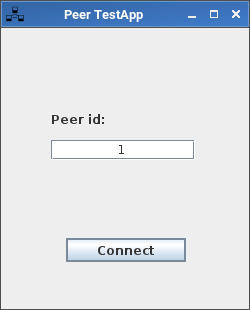
\includegraphics[scale=0.40]{TestApp.png}
    \caption{TestApp connection window}
    \label{fig:TestApp.png}
\end{figure}

\begin{figure}[h]
    \centering
    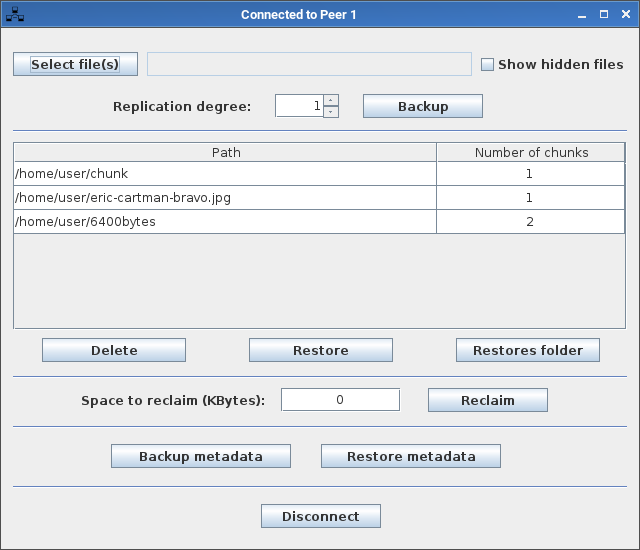
\includegraphics[scale=0.40]{ActionTester.png}
    \caption{ActionTester main window}
    \label{fig:ActionTester.png}
\end{figure}

\begin{figure}[h]
    \centering
    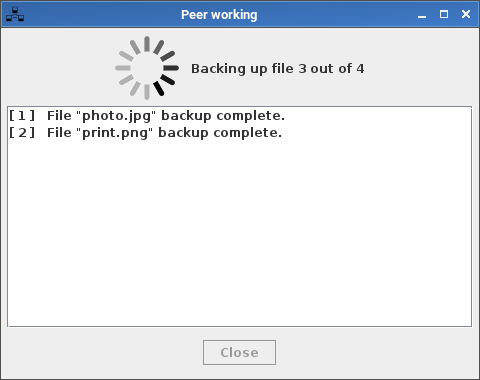
\includegraphics[scale=0.40]{PeerRequest.png}
    \caption{PeerRequest dialog with progress reports}
    \label{fig:PeerRequest.png}
\end{figure}

\begin{figure}[h]
    \centering
    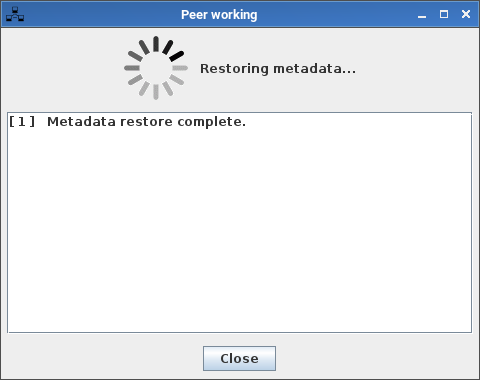
\includegraphics[scale=0.40]{MetadataRestoration.png}
    \caption{Meta-data restoration UI}
    \label{fig:MetadataRestoration.png}
\end{figure}

\clearpage
\section{Project development effort}

\subsection{Project development time estimations}
\begin{labeling}{alligator}
\item [\textbf{Inside classes}] 6 hours.
\item [\textbf{Outside classes}] 40 hours.
\item [\textbf{Total}] 46 hours.
\end{labeling}

\subsection{Individual contribution rates}
\begin{labeling}{alligator}
\item [\textbf{José Peixoto}] 80\%
\item [\textbf{Pedro Moura}] 18\%
\item [\textbf{Paulo Costa}] 1\%
\item [\textbf{Marina Camilo}] 1\%
\end{labeling}

\end{document}\grid
